%% nilHMM methods paper -- optimization supplement.
%% The C++/Rcpp reimplementation of the RTIGER and nNIL cores: a prerequisite for
%% simulation-scale calibration, established correctness-first (equivalence to the
%% Julia RTIGER), then throughput/memory. Structure mirrors the fork report
%% (faustovrz/RTIGER docs/optimization.md) reframed as C++/Rcpp vs Julia.
%% Compiles standalone or is \input into main.tex's \section*{Supplement}.
%% Section 1 (C++/Rcpp vs Julia) is FILLED from scripts/bench_rtiger_cpp_vs_julia.R
%% (writeup: analysis/rtiger-optimization-benchmark.qmd). Section 2 (nNIL) still has
%% \todo marks, pending the Zhong et al. panel (analysis/nnil-reproduction-benchmark.qmd).
\documentclass[11pt]{article}
\usepackage{amsmath,amssymb}
\usepackage{graphicx}
\usepackage[margin=1in]{geometry}
\usepackage{booktabs}
\usepackage{array}
\usepackage[round,authoryear]{natbib}
\usepackage[colorlinks=true,linkcolor=blue,urlcolor=blue,citecolor=blue]{hyperref}
\usepackage{xcolor}
\providecommand{\todo}[1]{{\footnotesize\textcolor{red}{[TODO: #1]}}}
\newcommand{\code}[1]{\texttt{#1}}
\newcommand{\bigO}{\mathcal{O}}
\newcommand{\states}{\lvert S\rvert}
\setlength{\emergencystretch}{3em}

\title{Supplemental Text: the C++/Rcpp reimplementation\\[2pt]
\large Simulation-calibrated HMM ancestry calling for near-isogenic lines\\
across sequencing modalities (nilHMM)}
\author{Rodr\'iguez-Zapata \textit{et al.}}
\date{}

\begin{document}
\maketitle

%======================================================================
\section{The C++/Rcpp reimplementation of the RTIGER and nNIL cores}
\label{supp:optimization}
%======================================================================

\begin{sloppypar}\hbadness=10000\relax
The named callers of the main text run on a single engine reimplemented in
C++/Rcpp (\code{nilhmm/src/}: \code{rtiger.cpp}, \code{viterbi\_batch.cpp},
\code{emission\_count.cpp}, \code{lbimpute.cpp}, \code{fsfhap.cpp}, and the shared
forward/backward and segment routines). This reimplementation removes the Julia
runtime that upstream RTIGER \citep{rtiger_2023} requires through
\code{JuliaCall}, and it makes a single fit cheap enough to loop over the
calibration sweeps and coverage sweeps of the main text at $10^4$ to $10^5$
markers on a laptop. We first establish its correctness, then report speed and
memory.
\end{sloppypar}

We benchmark the shipped C++/Rcpp core directly against the \emph{upstream
original} Julia RTIGER \citep{rtiger_2023} on one shared marker panel, at this
dataset's operating rigidity $r=250$: a Viterbi-identical equivalence oracle first,
then throughput and memory. The C++ core is measured at all five panel sizes; the
original Julia, being orders of magnitude slower, is measured at the three small
sizes and projected from their power-law fit to the two large sizes (its full
109{,}703-marker convergence fit is projected at about 1.3~hours).

\paragraph{Data.} Real \emph{Arabidopsis} Col-0 $\times$ Ler allele counts
(BioProject PRJNA720439 / SRA study SRP313911), the 109{,}703-locus panel of loci
covered in all three of the BN/Z/AU samples, thinned by odd index to five sizes
(6{,}857; 13{,}713; 27{,}426; 54{,}852; 109{,}703 markers per sample). Both cores
were run from the identical deterministic initialization ($\alpha=[20,20,1]$,
$\beta=[1,20,20]$, diagonal-dominant transition, uniform start), rigidity~$250$ (the
operating value for this \emph{Arabidopsis} panel; every chromosome chain exceeds
the required $2r=500$ covered markers at all five sizes), \code{eps}~$=0.01$.
Compute: \code{scripts/bench\_rtiger\_r250.R} (C++, all sizes) and
\code{scripts/rtiger\_julia\_conv\_worker.jl} (original, small sizes). The
nNIL reproduction (Sec.~\ref{supp:nnil}) uses the Zhong \emph{et al.} nested-NIL
panel.

\paragraph{Environment.} All timings are wall-clock on an Apple M4 (10 cores,
24~GB RAM), macOS~26.5 (\code{arm64}), single-threaded (\code{threads}~$=1$). The
nilHMM C++/Rcpp core was built native \code{arm64} with Apple clang~17
(\code{-std=gnu++17 -O2}); R~4.5.2, nilHMM~0.3.0, Rcpp~1.1, RcppParallel~5.1.11.
Its forward/backward, Viterbi, and emission M-step are hand-written scalar C++
(\code{LinkingTo}: only Rcpp and RcppParallel; no Armadillo, Eigen, or external
BLAS/LAPACK), so the system linear-algebra library cannot affect these timings.
C++ throughput points are the median of three fits. The upstream-original Julia
RTIGER baseline (Julia~1.12.6) was run on the same hardware at $r=250$ for the three
small sizes; its two large sizes are projected from the power-law fit. The full
environment is recorded per run in \code{results/bench/rtiger\_env.txt}.

%----------------------------------------------------------------------
\subsection{Where the cost goes: a complexity analysis}
\label{supp:complexity}
%----------------------------------------------------------------------
Before the measurements we account, step by step, for the asymptotic cost of the
rigid-HMM Baum--Welch fit and for the factor each optimization removes. Every
optimization preserves the arithmetic of the model \citep{rtiger_2023}; only the
cost of evaluating it changes. Table~\ref{tab:cost-symbols} fixes notation.

\begin{table}[htbp]
\centering
\small
\begin{tabular}{@{}c l@{}}
\toprule
symbol & meaning \\
\midrule
$T$        & markers (positions) in one observation chain \\
$C$        & chains (samples $\times$ chromosomes); $T_{\text{tot}}=\sum_c T_c$ \\
$N$        & number of samples (so $C$ and $T_{\text{tot}}$ grow $\propto N$) \\
$s=\states$ & hidden states ($=3$: paternal / heterozygous / maternal) \\
$r$        & rigidity; augmented rigid space $S'=S\times\{1,\dots,r\}$, $\lvert S'\rvert=s\,r$ \\
$D$        & number of \emph{distinct} emission pairs $(k,n)$ in a chain \\
$E$        & objective evaluations per state in one emission-M-step line search \\
\bottomrule
\end{tabular}
\caption{Cost parameters. For low-coverage genotyping the read depth $n$ is small,
so the distinct $(k,n)$ pairs number a few dozen regardless of $T$: $D\ll T$.}
\label{tab:cost-symbols}
\end{table}

The emission is a Beta--Binomial in the read counts,
$\psi_s(k;n,a_s,b_s)=\binom{n}{k}\,\mathrm{B}(k+a_s,\,n-k+b_s)/\mathrm{B}(a_s,b_s)$,
whose evaluation costs a handful of \code{lgamma} calls, the dominant scalar
operation of the fit. A full fit costs
$(\#\text{EM iters})\times\sum_{c}(\text{E-step}_c+\text{M-step}_c)$, so we analyse
the per-iteration, per-chain cost. Throughout, the upstream original is the
``before'' and the nilHMM C++/Rcpp core the ``after''; every step below is realized
in the shipped core (\code{nilhmm/src/rtiger.cpp}).

\paragraph{Windowed emission product ($\Psi$).} The rigid recursions repeatedly need
the windowed product $\Psi^t_k=\prod_{u=\max(t-r+1,1)}^{t}\psi_k(o_u)$. Recomputing
each of the $T s$ values over its length-$r$ window costs $\bigO(T s r)$; in log
space it is a fixed-width sliding sum (add the entering term, drop the leaving term,
$\bigO(1)$ per step), giving $\bigO(T s r)\to\bigO(T s)$ and removing the rigidity
factor $r$.

\paragraph{Emission log-pdf memoization.} Each forward, backward and Viterbi step
needs $\psi_s(o_t)$ at every position, but $\psi_s$ depends on $o_t=(k_t,n_t)$ only,
and there are just $D$ distinct pairs. Memoizing $\log\psi_s$ over the distinct
$(k,n)$ turns $\bigO(T s)$ Beta--Binomial evaluations into $\bigO(D s)$ evaluations
plus $\bigO(T s)$ table lookups: the costly part shrinks by the factor $T/D$.

\paragraph{Emission M-step line search (the dominant cost).} The Beta--Binomial
parameters are fit by a 1-D line search over the concentration $\tau_s$ at the
empirical mean $m_s$ ($a_s=m_s\tau_s$, $b_s=(1-m_s)\tau_s$), maximizing
$Q(\tau_s)\propto\sum_{c}\sum_{t}\gamma^{t,c}_s\,\log\psi_s(k^c_t;n^c_t,a_s,b_s)$.
\emph{Upstream}, each of the $E$ line-search evaluations rebuilds a Beta--Binomial
and sums over all $T_{\text{tot}}$ markers: $\bigO(E\,s\,T_{\text{tot}})$ per
iteration, which is empirically the bulk of upstream runtime and makes the fit
super-linear. \emph{In the C++/Rcpp core} the sum is regrouped once, because it
depends on the data only through the $\gamma$-weighted counts at each distinct pair:
\[
Q(\tau_s)=\sum_{(k,n)\in\mathcal D}\underbrace{\Big(\textstyle\sum_{t:\,(k_t,n_t)=(k,n)}\gamma^{t}_s\Big)}_{G_s(k,n)\ \text{(pre-summed once)}}\;\log\psi_s(k;n,a_s,b_s).
\]
The weights $G_s(k,n)$ accumulate in one $\bigO(s\,T_{\text{tot}})$ pass; each
line-search evaluation then costs $\bigO(s\,D)$, so
$\bigO(E\,s\,T_{\text{tot}})\to\bigO(s\,T_{\text{tot}}+E\,s\,D)$. Since
$E\,D\ll T_{\text{tot}}$, the M-step collapses from ``$E$ passes over all markers,
rebuilding objects'' to ``one binning pass,'' and is no longer the bottleneck.

\paragraph{Forward/backward and Viterbi.} The rigid forward, backward and Viterbi
each take a $\max$/sum over $s$ predecessors at every position: $\bigO(T s^2)$ per
chain (the dwell-counter shifts are $\bigO(1)$ once $\Psi$ is available). The C++
kernels use in-place scalar log-sum-exp and an allocation-free arg-max, a
constant-factor win that leaves the class unchanged. \emph{Once the M-step above is
regrouped, these $\bigO(T s^2)$ kernels are what the per-iteration cost reduces to},
hence linear in $T$.

\paragraph{Memory: streaming the sufficient statistics.} The M-step needs the data
only through pooled sums over chains: the $s\times s$ transition counts
$\sum_c\zeta$, the start counts $\sum_c\gamma^{1}$, and the weighted counts
$G_s(k,n)$. Holding, for all $C$ chains at once, the per-chain arrays $\zeta$
($T\times s^2$), the posteriors $\gamma,\alpha,\beta$ ($s\times T$) and the windowed
emission product $\psi$ ($s\times(T+r)$) costs $\bigO(N\,T\,s^2)$, linear in the
sample count $N$. Folding each chain's contribution into the running sums inside the
E-step and discarding its arrays immediately makes peak scratch one chain's worth,
$\bigO(T_{\max}\,s^2)+\bigO(T_{\text{tot}})$, independent of $N$: a population-scale
joint fit stays within a workstation's memory.

\paragraph{Parallelism.} The E-step is independent across chains (the M-step only
pools their summed statistics), so with $P$ threads the per-iteration wall time is
$\bigO(T s^2)\to\bigO(T s^2/P)$: the constant drops by $P$ but the exponent is
unchanged (a bounded thread pool is a constant-factor speed-up, not a
complexity-class change). A fixed-order reduction keeps the result deterministic;
\code{threads}~$=1$ is the bit-identical serial path.

\begin{table}[htbp]
\centering
\small
\renewcommand{\arraystretch}{1.25}
\begin{tabular}{@{}l l l l@{}}
\toprule
optimization & before (per iter) & after (per iter) & effect \\
\midrule
$\Psi$ window          & $\bigO(T s r)$              & $\bigO(T s)$                          & drop $r$ \\
emission log-pdf       & $\bigO(T s)$ evals         & $\bigO(D s)$ evals                    & factor $T/D$ \\
emission M-step        & $\bigO(E s T_{\text{tot}})$ & $\bigO(s T_{\text{tot}}+E s D)$      & removes the per-marker pass \\
forward/backward       & $\bigO(T s^2)$             & $\bigO(T s^2)$                        & constant factor \\
Viterbi                & $\bigO(T s^2)$             & $\bigO(T s^2)$                        & constant factor \\
\midrule
memory (streaming)     & $\bigO(N T s^2)$   & $\bigO(T_{\max}\,s^2)$          & drop $N$ \\
\bottomrule
\end{tabular}
\caption{Per-EM-iteration time complexity (top) and peak-memory complexity
(bottom) of the upstream original vs the nilHMM C++/Rcpp core. $s=3$ is constant;
the asymptotically meaningful factors are $T$, $r$, $D$, $E$ and $N$.}
\label{tab:complexity}
\end{table}

Crucially, the rigidity is implemented in \emph{collapsed} form (the window product
above plus an $r$-step transition offset, not an explicit $s\times r$ dwell-state
enumeration), so the optimized core's per-iteration time and memory are essentially
independent of $r$: the recursion stays $\bigO(T s^2)$ and $r$ enters only as the
$\bigO(s r)$ tail of the $\Psi$ buffer. The upstream original, by contrast,
recomputes each length-$r$ window at $\bigO(T s r)$, so at this dataset's operating
rigidity ($r=250$) the $\Psi$-window win is a first-order effect rather than a
footnote, on top of the M-step regrouping and the sample-scaling memory win from
streaming. These asymptotics are what the measured scaling confirms next: the C++
per-iteration cost is the $\bigO(T s^2)$ kernels, linear in $T$
(Sec.~\ref{supp:throughput}).

%----------------------------------------------------------------------
\subsection{Equivalence to Julia RTIGER (correctness first)}
%----------------------------------------------------------------------
Both cores were run to full convergence from the identical deterministic
initialization at $r=250$ and compared position by position, at the three sizes we
run the original (Table~\ref{tab:cpp-equiv}). At every size the two cores take the
\emph{same} number of EM iterations, impute \emph{identical} ancestry states at
every marker position across all three samples (0 mismatches), and fit emission
parameters agreeing to $\le 3.1\times10^{-6}$, float-summation order, not an
algorithmic difference. Correctness is rigidity-independent, as expected for a
bit-identical port: the full 109{,}703-marker panel run at $r=2$ likewise gives 0
mismatches (329{,}109 of 329{,}109 states). Their per-iteration EM convergence
trajectories coincide on the $1{:}1$ line (Fig.~\ref{fig:cpp-equiv}, right): the
plotted $\delta$ is the \emph{EM parameter delta}, the maximum absolute change in
the BetaBinomial emission parameters $(\alpha,\beta)$ between successive EM
iterations, i.e.\ RTIGER's convergence criterion, not a log-likelihood change.

\begin{table}[htbp]
\centering
\small
\begin{tabular}{@{}r c c c c@{}}
\toprule
markers / sample & EM iters (C++ / Julia) & Viterbi match & mismatches & param max-diff \\
\midrule
6{,}857   & 3 / 3 & 20{,}571 / 20{,}571 & 0 & $4\times10^{-7}$ \\
13{,}713  & 3 / 3 & 41{,}139 / 41{,}139 & 0 & $6\times10^{-7}$ \\
27{,}426  & 4 / 4 & 82{,}278 / 82{,}278 & 0 & $3.1\times10^{-6}$ \\
\bottomrule
\end{tabular}
\caption{nilHMM C++/Rcpp vs upstream-original Julia RTIGER at rigidity $r=250$, run
to convergence from the identical deterministic init, at the three small sizes we
run the original. The \emph{Viterbi match} and \emph{mismatches} columns count the
imputed ancestry states (REF/HET/ALT, one per marker) on which the two cores agree,
respectively differ, pooled over every position in all three samples (total =
(markers/sample)~$\times\,3$). At every size the two cores take the identical EM
iteration count, impute identical ancestry at every position (0 mismatches), and fit
emission parameters to float-summation tolerance; the full 109{,}703-marker panel at
$r=2$ likewise gives 0 mismatches. Compute: \code{scripts/bench\_rtiger\_r250.R}.}
\label{tab:cpp-equiv}
\end{table}

\begin{figure}[htbp]
\centering
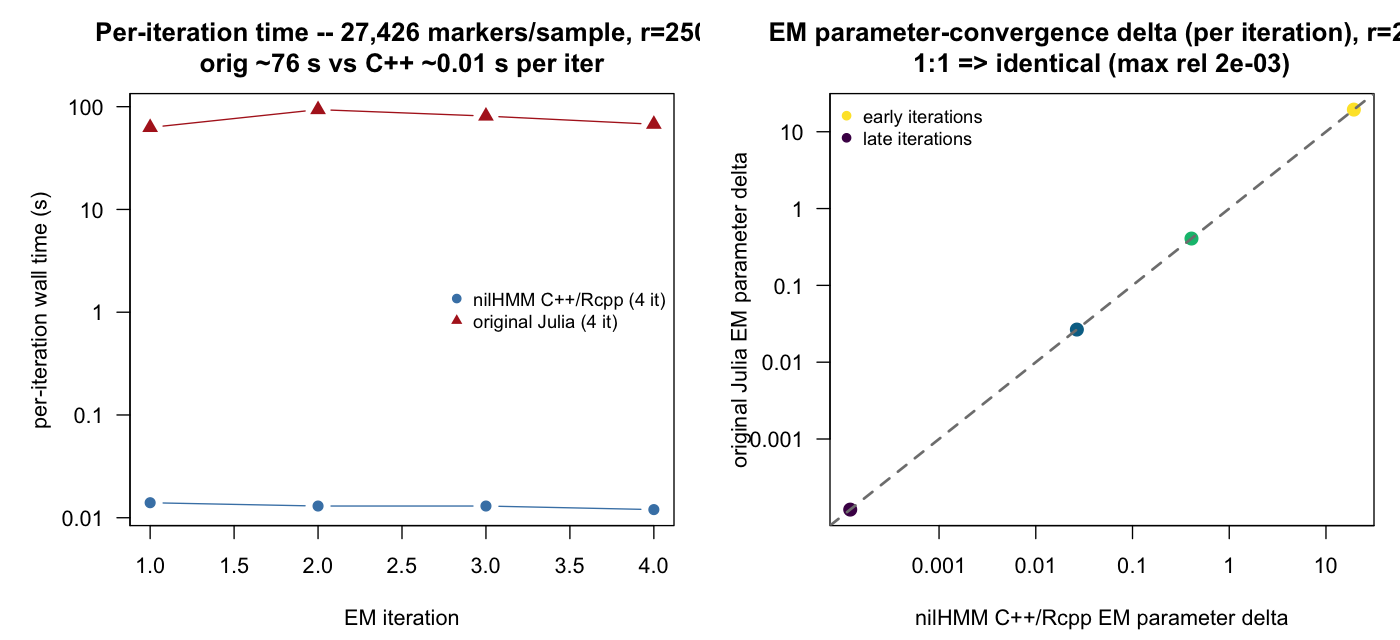
\includegraphics[width=\textwidth]{figures/rtiger_equivalence_r250.png}
\caption{Largest measured size (27{,}426 markers/sample), rigidity $r=250$, both
cores run to convergence (4 iterations each). \textbf{Left:} per-iteration wall
time, original Julia ($\sim$76~s/iter, dominated by its recomputed length-$r$
emission window) vs nilHMM C++/Rcpp ($\sim$0.01~s/iter, flat). \textbf{Right:} each
iteration's \emph{EM parameter delta} (the maximum absolute change in the
BetaBinomial emission parameters $(\alpha,\beta)$ between successive EM iterations,
i.e.\ RTIGER's convergence criterion, not a log-likelihood change), C++ against
original Julia on a log-log $1{:}1$ line (max relative difference
$2\times10^{-3}$), early (yellow) to late (purple). The left panel illustrates the
speed optimization; the right illustrates the faithful reproduction, the two cores
descending the identical path to convergence.}
\label{fig:cpp-equiv}
\end{figure}

%----------------------------------------------------------------------
\subsection{Throughput and memory}
\label{supp:throughput}
%----------------------------------------------------------------------
On a log-log plot the per-iteration wall time against markers per sample is a
straight line whose slope is the empirical complexity exponent
(Fig.~\ref{fig:cpp-scaling}, left). At $r=250$ the upstream original scales as
markers$^{1.77}$, its cost now split between the emission M-step and the
$\bigO(T s r)$ recomputed length-$r$ emission window. The C++/Rcpp core scales as
markers$^{1.03}$, essentially linear, the $\bigO(T s^2)$ kernels of
Sec.~\ref{supp:complexity} once the M-step is regrouped and the window is a sliding
sum. The full-fit speed-up is $\sim$2{,}000$\times$ at the smallest size, widening to
a projected $\sim$22{,}000$\times$ at the full panel (Table~\ref{tab:cpp-speed}),
which makes the calibration and coverage sweeps of the main text tractable.

Memory separates the two the same way (Fig.~\ref{fig:cpp-scaling}, right). The C++
E-step streams each chain into fixed-size pooled sufficient statistics and never
retains the per-sample \code{zeta}/\code{gamma}/\code{alpha}/\code{beta} arrays
(Sec.~\ref{supp:complexity}), whereas the original holds them for every sample. On
the shared panel the C++ core uses $\sim$5--6$\times$ less resident memory
($\sim$140--201~MiB vs $\sim$815--894~MiB); both are near-flat in markers here
because only three samples are held, but the C++ scratch is $\bigO(T_{\max}\,s^2)$
rather than $\bigO(N\,T\,s^2)$, so the gap widens with sample count: a
population-scale joint fit stays within a workstation's memory where the
array-retaining original would not.

\begin{figure}[htbp]
\centering
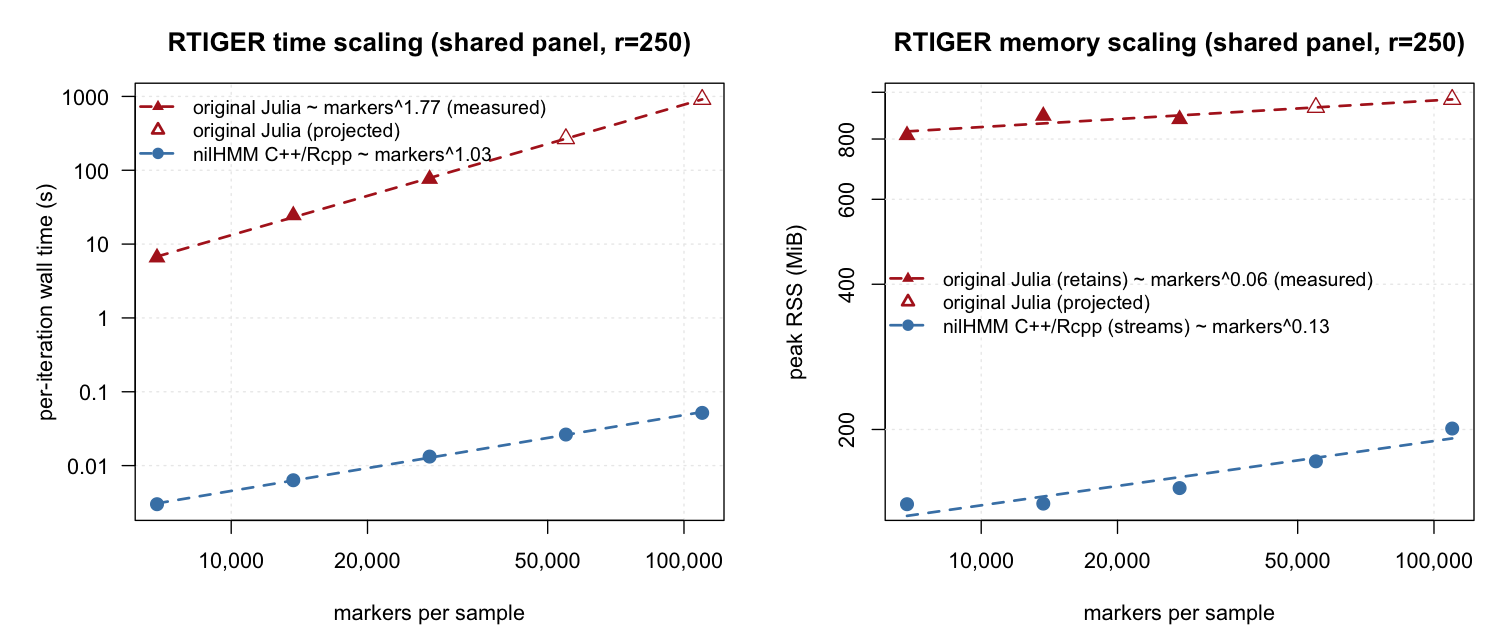
\includegraphics[width=\textwidth]{figures/rtiger_marker_scaling_r250.png}
\caption{RTIGER scaling on the shared \emph{Arabidopsis} panel at rigidity $r=250$,
original array-retaining Julia vs nilHMM C++/Rcpp. Filled symbols are measurements
(C++ at all five sizes, original at the three small ones); open red symbols are the
original projected from its power-law fit; dashed lines are the fits.
\textbf{Left:} per-iteration wall time (original $\sim$markers$^{1.77}$; C++
$\sim$markers$^{1.03}$, linear). \textbf{Right:} peak resident memory; the C++ core
streams sufficient statistics and stays $\sim$5--6$\times$ lower. Compute:
\code{scripts/rtiger\_r250\_plot.R}.}
\label{fig:cpp-scaling}
\end{figure}

\begin{table}[htbp]
\centering
\small
\begin{tabular}{@{}r r r r@{}}
\toprule
markers / sample & original Julia & nilHMM C++/Rcpp & speed-up \\
\midrule
6{,}857   & 19.7~s                    & 0.009~s & $\sim$2{,}200$\times$ \\
13{,}713  & 73.6~s                    & 0.019~s & $\sim$3{,}900$\times$ \\
27{,}426  & 305~s                     & 0.053~s & $\sim$5{,}800$\times$ \\
54{,}852  & $\sim$1{,}180~s (proj.)              & 0.079~s & $\sim$15{,}000$\times$ \\
109{,}703 & $\sim$4{,}630~s (proj., $\sim$1.3~h) & 0.207~s & $\sim$22{,}000$\times$ \\
\bottomrule
\end{tabular}
\caption{Full-fit wall time to convergence (3 samples, \code{eps}~$=0.01$, rigidity
$r=250$, native arm64), original Julia vs nilHMM C++/Rcpp. The original's two
largest sizes are projected from the power-law fit of the three measured sizes
(marked ``proj.''). The speed-up grows with problem size because the C++ core is
near-linear (Fig.~\ref{fig:cpp-scaling}).}
\label{tab:cpp-speed}
\end{table}

%======================================================================
\section{Reproduction of the nested-NIL HMM (nNIL)}
\label{supp:nnil}
%======================================================================
nilHMM's \code{nNIL} caller (categorical genotype-confusion emission, geometric
duration) reimplements Holland's nested-NIL HMM \citep{zhong2025}. The
reimplementation is faithful by construction: the $3\times4$ emission matrix (three
ancestry states $\times$ \{REF, het, donor, missing\} calls) is transcribed
verbatim from the original Python (\code{File\_S11}, an \code{hmmlearn}
\code{MultinomialHMM}), and the transition uses the identical frequency-weighted
parameterization (self-stay $1-r$; off-diagonals split by the expected state
frequencies $f_0, f_1, f_2$; start $[f_0, f_1, f_2]$). We verify that faithfulness
directly, running both cores on the same genotypes and comparing calls
position-by-position.

\paragraph{Data.} The full Zhong \emph{et al.} nNIL population: File S1 raw GBS
genotypes put through Holland's own \code{File\_S10} filter, which reproduces his
filtered genotype table exactly (888 nested-NIL lines $\times$ 64{,}025 markers, 0
cell differences), recoded \{REF, het, donor, missing\} $\to$
\{0,1,2,3\}, giving 56{,}854{,}200 genotype states. Both cores were run from the
published operating point (File S16: \code{nir}$=0.9$, \code{germ}$=0.01$,
\code{gert}$=10^{-4}$, $p=0.9$, $f_1=0.00781$, $f_2=0.01118$, $r=4.7\times10^{-4}$).
Compute: \code{scripts/nnil\_equiv/}.

%----------------------------------------------------------------------
\subsection{Equivalence to the original Python}
%----------------------------------------------------------------------
We decode the full population with both cores at seven marker densities (odd-index
thinning of the 64{,}025-marker panel, as in the RTIGER sweep), from identical
thinned genotypes and the identical per-size transition rate, and compare the calls
position by position (Table~\ref{tab:nnil-equiv}). At \emph{every} density the two
cores agree at \emph{every} informative (homozygous) marker (0 informative-marker
mismatches throughout, the exactness test). The only differences, a handful out of
tens of millions of states (1 at the full panel, at most $\sim$100 at the sparsest),
fall exclusively at missing and heterozygous positions, where two ancestry states
are emission-equal and any Viterbi difference is a boundary tie-break, not a
decoding disagreement. Holland's own re-run reproduces the \emph{published} File S18
calls exactly (0 mismatches), confirming the input is byte-identical to his.

\begin{table}[htbp]
\centering
\small
\begin{tabular}{@{}r c r r r@{}}
\toprule
markers / line & Viterbi match / states & mismatches & mismatch rate & at informative markers \\
\midrule
64{,}025 & 56{,}854{,}199 / 56{,}854{,}200 & 1   & $1.8\times10^{-8}$ & 0 \\
32{,}013 & 28{,}427{,}540 / 28{,}427{,}544 & 4   & $1.4\times10^{-7}$ & 0 \\
16{,}007 & 14{,}214{,}197 / 14{,}214{,}216 & 19  & $1.3\times10^{-6}$ & 0 \\
8{,}004  & 7{,}107{,}539 / 7{,}107{,}552   & 13  & $1.8\times10^{-6}$ & 0 \\
4{,}002  & 3{,}553{,}756 / 3{,}553{,}776   & 20  & $5.6\times10^{-6}$ & 0 \\
2{,}001  & 1{,}776{,}784 / 1{,}776{,}888   & 104 & $5.9\times10^{-5}$ & 0 \\
1{,}001  & 888{,}848 / 888{,}888           & 40  & $4.5\times10^{-5}$ & 0 \\
\bottomrule
\end{tabular}
\caption{nilHMM \code{nNIL} vs Holland's original Python (\code{hmmlearn}) on the
full Zhong \emph{et al.} nNIL population (888 lines), over an odd-index
marker-density sweep of the 64{,}025-marker panel, both cores run on the same
\code{File\_S10}-filtered genotypes and the identical per-size transition rate. The
\emph{Viterbi match / states} column gives the agreeing ancestry states
(REF/het/donor) out of the total, (markers/line)~$\times$~888, pooled over every
position; \emph{mismatches} is the disagreeing count and \emph{mismatch rate} its
fraction of the total. At every density the two
cores are identical at every informative (homozygous) marker (0 in the last column);
the few total differences fall only at missing and heterozygous positions, where the
states are emission-equal. Compute: \code{scripts/nnil\_equiv/07\_equiv\_sweep.R}.}
\label{tab:nnil-equiv}
\end{table}

%----------------------------------------------------------------------
\subsection{Throughput and memory}
%----------------------------------------------------------------------
Both callers were run on the same memory-mapped PLINK \code{.bed} input, over an
odd-index marker-density sweep of the full 888-line population
(Fig.~\ref{fig:nnil-scaling}). At the full 64{,}025 markers nilHMM decodes the
population in $\sim$4~s against $\sim$20~s for the \code{hmmlearn} caller (roughly
$5\times$ faster), with both times scaling near-linearly in marker count. Peak
memory separates the two: nilHMM streams one line at a time from the memory-mapped
\code{.bed} and holds $0.8$~GiB, whereas \code{hmmlearn} reads the whole genotype
matrix and reaches $2.3$~GiB, the gap widening with marker density.

\begin{figure}[htbp]
\centering
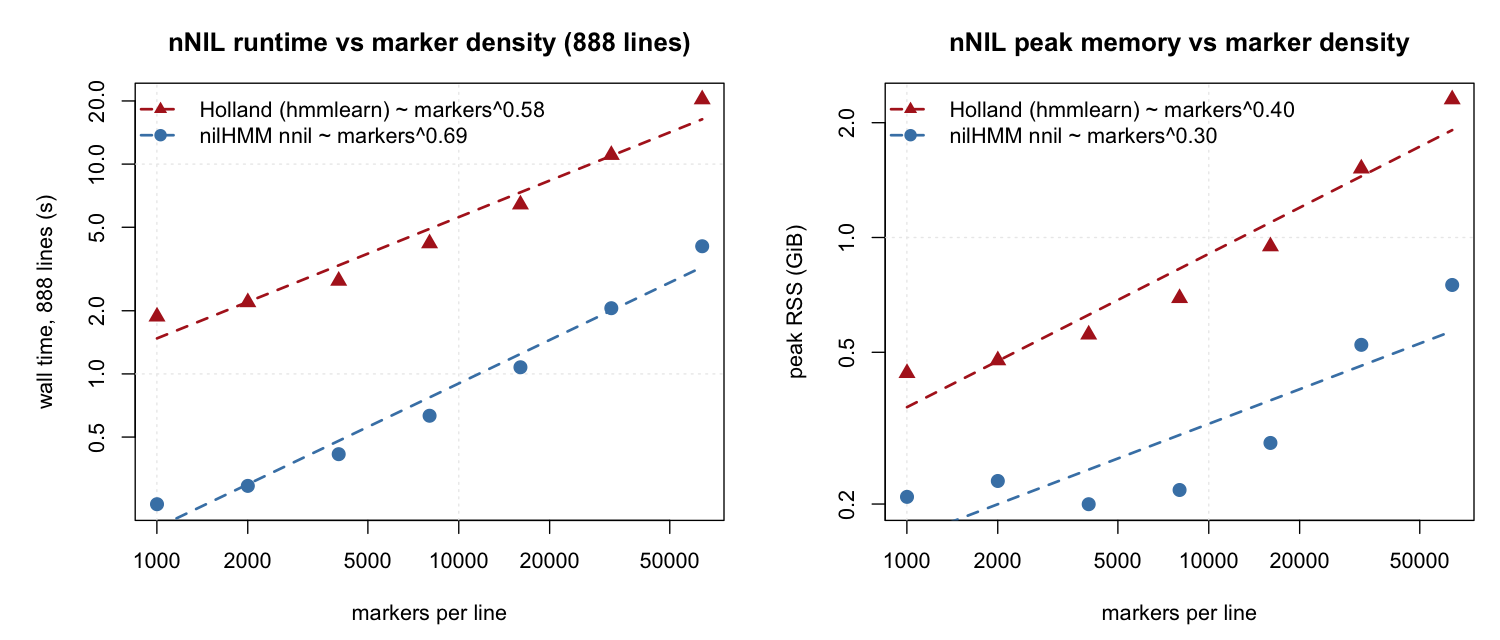
\includegraphics[width=\textwidth]{figures/nnil_marker_scaling.png}
\caption{nNIL caller scaling with marker density over the full 888-line population
(odd-index thinning of the 64{,}025-marker panel, shared memory-mapped
\code{.bed}). \textbf{Left:} wall time (log-log, power-law fits); the C++/Rcpp
\code{nNIL} is $\sim$5$\times$ faster. \textbf{Right:} peak resident memory; nilHMM
streams rows and stays low while the \code{hmmlearn} caller holds the full matrix
and the gap widens. Compute: \code{scripts/nnil\_equiv/06\_sweep.R}.}
\label{fig:nnil-scaling}
\end{figure}

\bibliographystyle{plainnat}
\bibliography{references}

\end{document}
